\section{Adding the frame class}

Some of the previous passes potentially add new local variables to the method. \textit{Renaming variables to unique
names} adds new variables by renaming the ones which could generate name clashes in this pass.
\textit{Replacing \code{foreach} loops with \code{for} loops} adds a new \code{iterator} variable for iterator-based
\code{foreach} loops and an index variable \code{i} for array-based \code{foreach} loops. If there is already a local
variable named \code{iterator} or \code{i}, in the method body, the pass generates a unique variable name by appending
indexes to these names, to avoid name clashes. The third pass which may add new local variables is
\textit{Extracting recursive calls to statements}, because the recursive calls are extracted to local variable
declaration statements named \code{temp}, with potential name clashes being again avoided with indexes, if necessary.

This pass generates a \code{private static} nested class named by the capitalized name of the method followed by the
\code{Frame} suffix. The fields of the frame class represent the variables of the method (both formal parameters and
local variables) which are relevant after a recursive call (whose scope contains at least a recursive call). They are
declared as \code{private}, because the enclosing class can still access the fields of this class. The frame class also
contains a \code{private} constructor which initializes only the fields representing the formal parameters of the
method, because the fields corresponding to local variables are initialized by assignment in the method body,
after another pass. Until they are initialized in the method body, they have the corresponding default values.
By virtue of \textit{Definite Assignment}\footnote{\url{https://docs.oracle.com/javase/specs/jls/se8/html/jls-16.html}},
provided that the method compiles without errors before the refactoring, there will not be any problems involving using
uninitialized local variables.

There is an additional \code{int} field named \code{block} in the frame class, which represents the index of the
block of code to which the method jumps when returning from the callee to continue executing the statements in the
caller after the recursive call.

An example of a frame class in provided in \labelindexref{Figure}{img:add-frame-class}.
The frame class contains the formal parameters of the method as fields. The field \code{iterator} has been generated
because the \code{foreach} loop has been converted to a \code{for} loop, since it contains a recursive call. The
variable \code{n} is added as a corresponding field to the frame class, because its scope contains a recursive call.
On the other hand, the local variable \code{ctc} does not have a corresponding field in the frame class, because its
scope does not include a recursive call. Finally, the \code{block} field is added to the fields of the frame class.

\begin{figure}[htb]
    \makebox[\linewidth][c]{%
    \begin{subfigure}[b]{.5\textwidth}
        \centering
        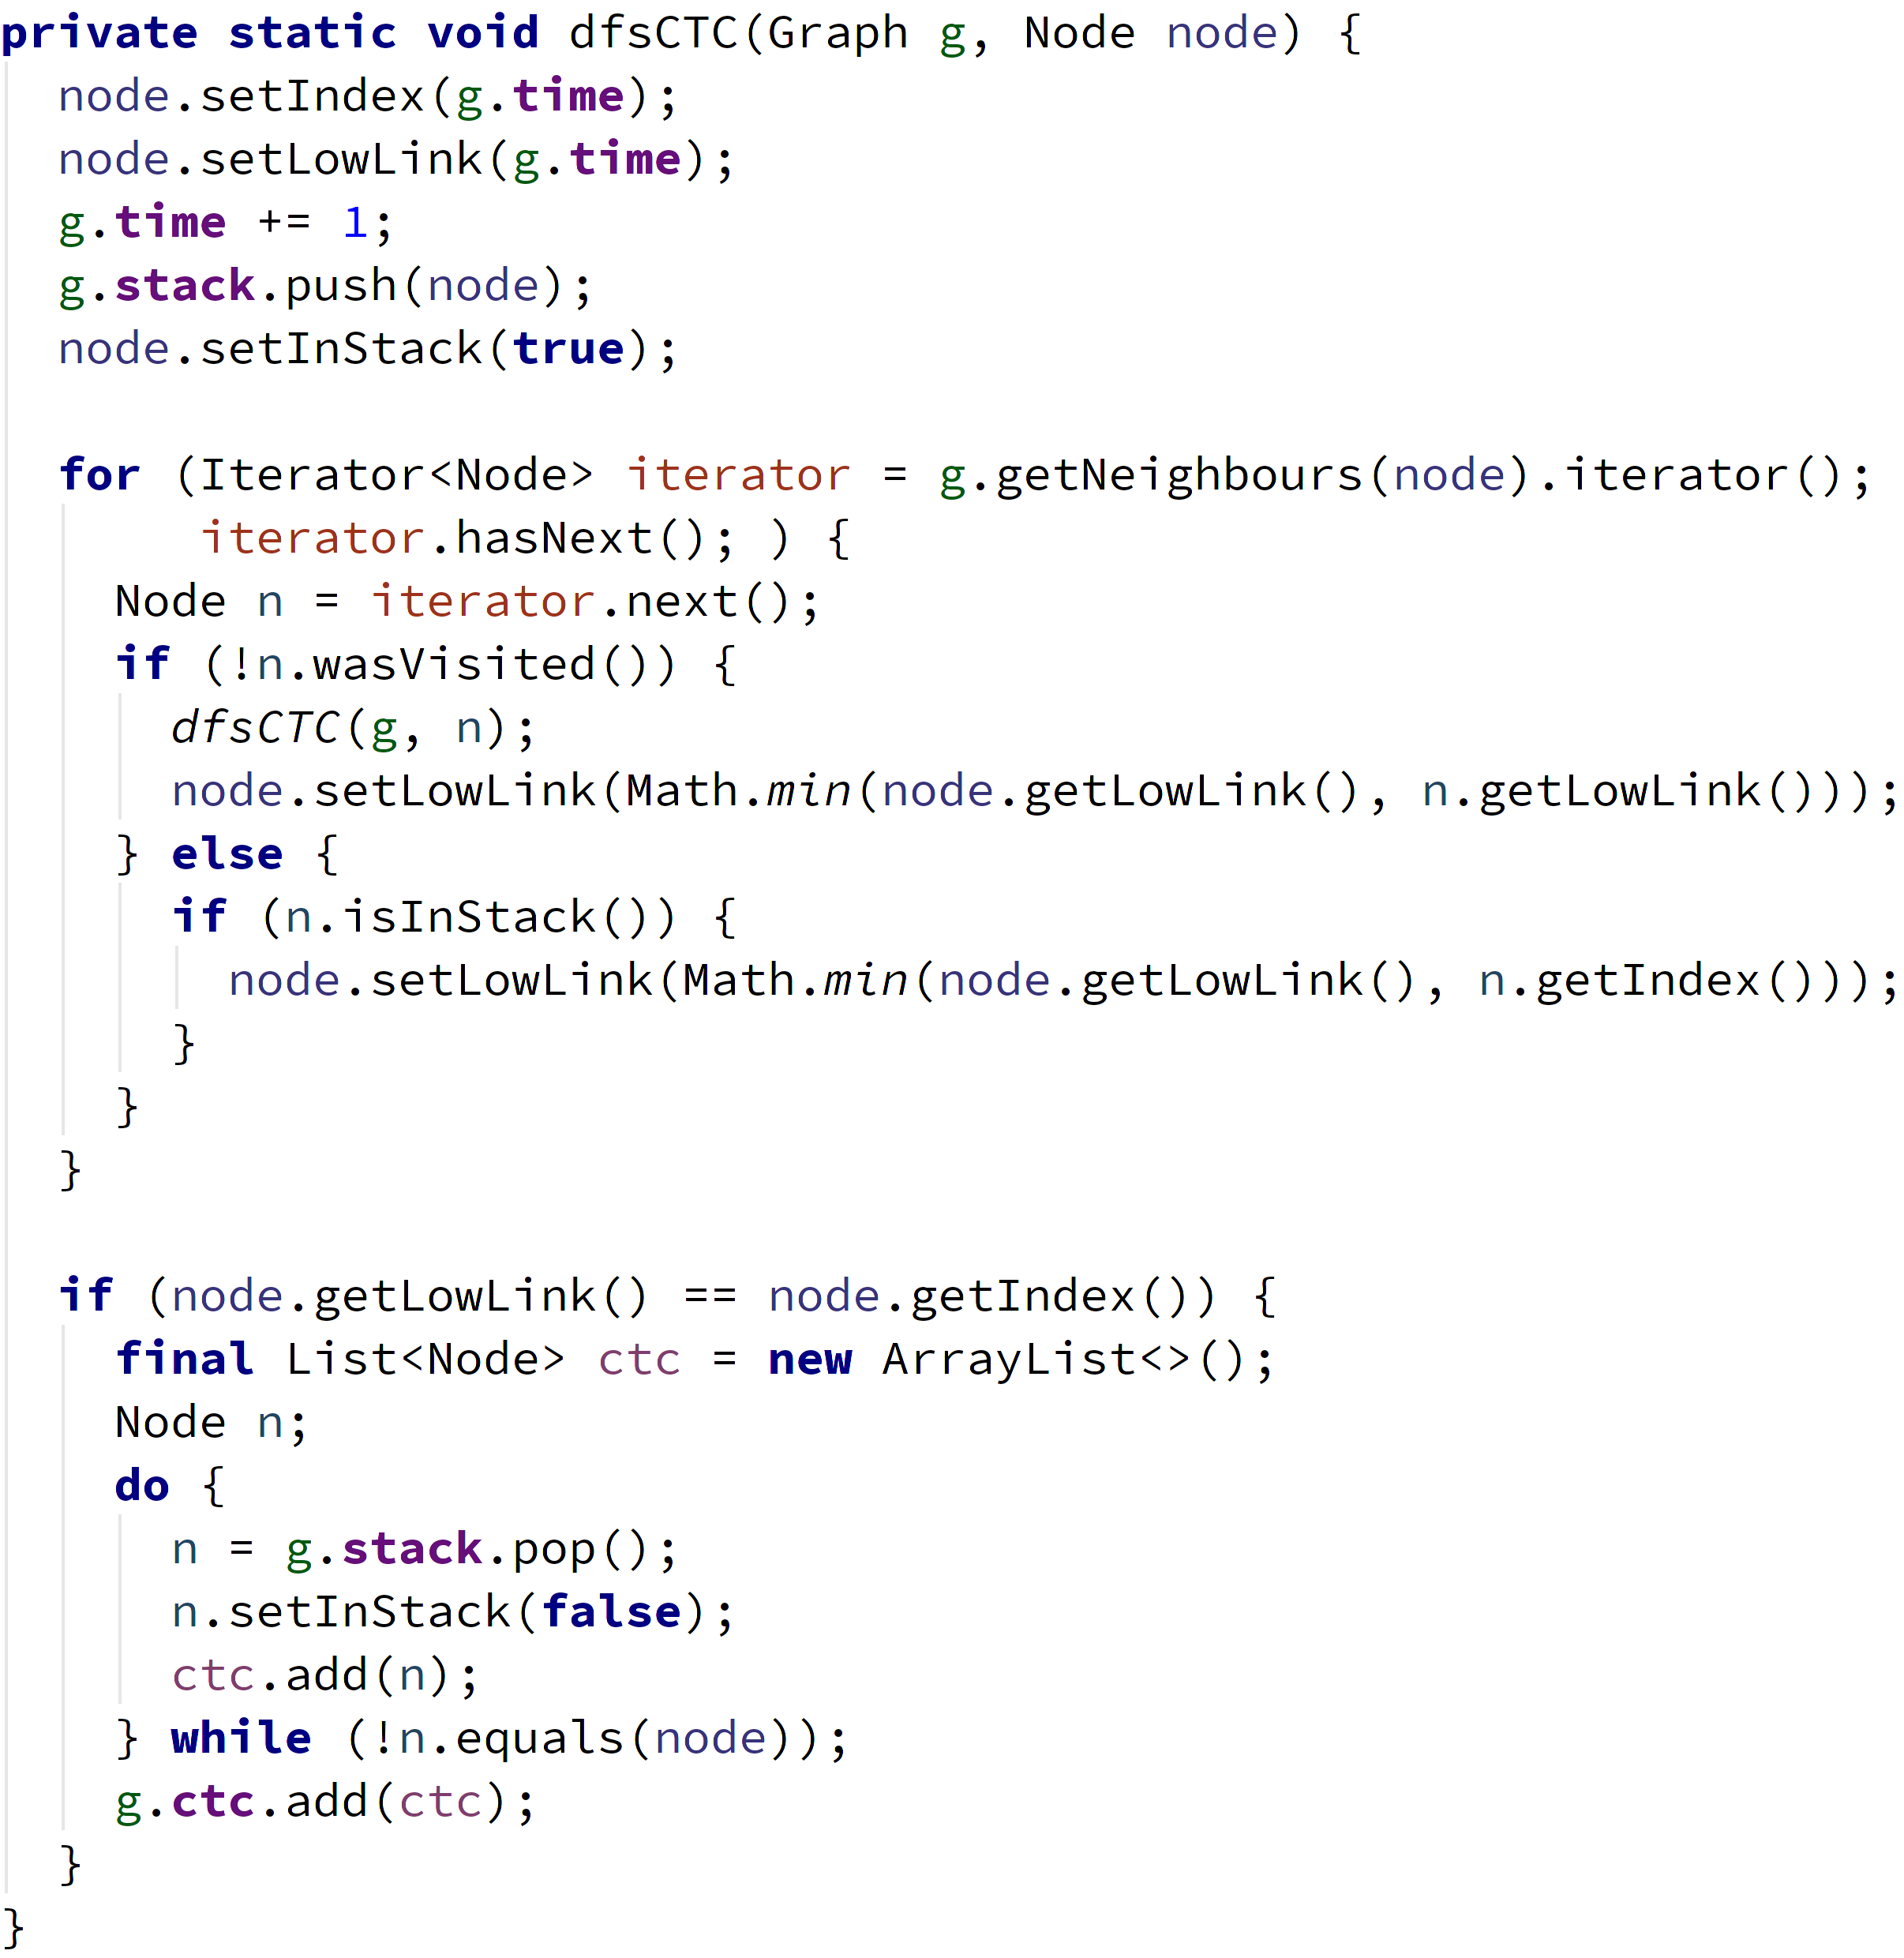
\includegraphics[height=2.5in]{src/img/add-frame-class-before-white-31.png}
        \caption{Before}
    \end{subfigure}%
    \begin{subfigure}[b]{.5\textwidth}
        \centering
        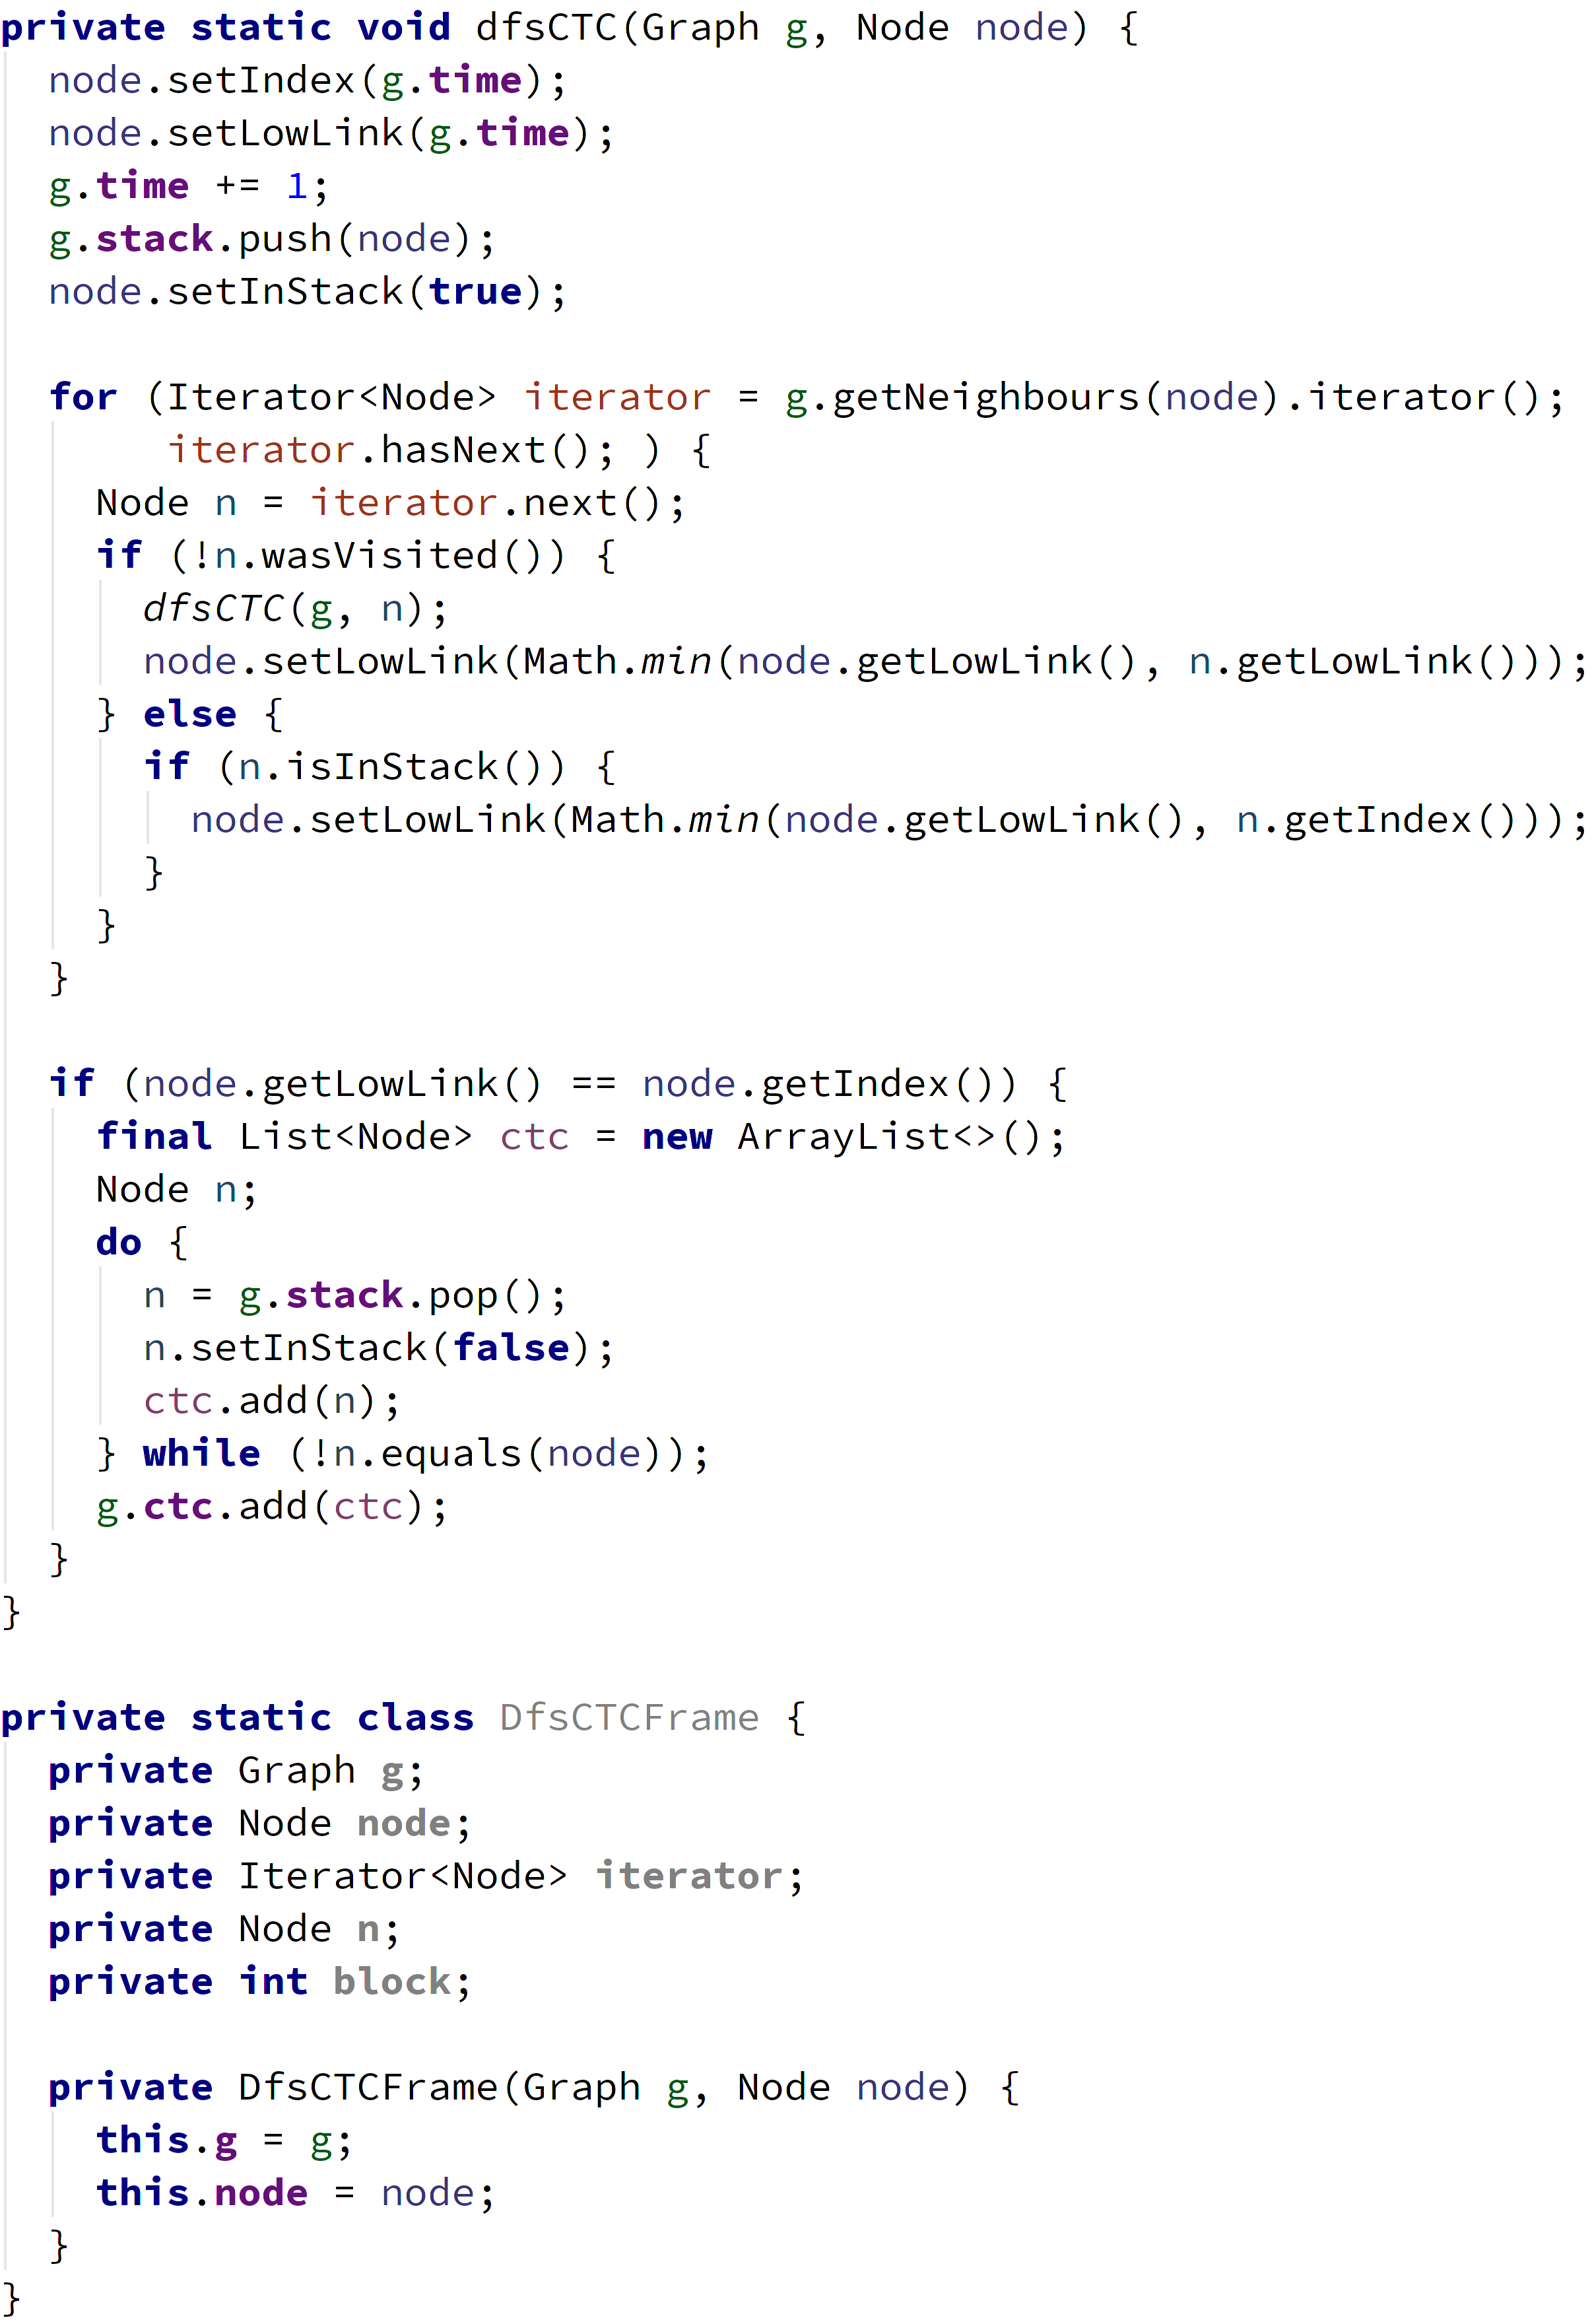
\includegraphics[height=3.548in]{src/img/add-frame-class-after-white-44.png}
        \caption{After}
    \end{subfigure}%
    }\\
    \caption{Adding the frame class \label{img:add-frame-class}}
\end{figure}